\documentclass[12pt,a4paper]{article}
\usepackage{ctex}
\usepackage{amsmath,amscd,amsbsy,amssymb,latexsym,url,bm,amsthm}
\usepackage{epsfig,graphicx,subfigure}
\usepackage{enumitem,balance}
\usepackage{wrapfig}
\usepackage{mathrsfs,euscript}
\usepackage[usenames]{xcolor}
\usepackage{hyperref}
\usepackage[vlined,ruled,linesnumbered]{algorithm2e}
\usepackage{array}
\hypersetup{colorlinks=true,linkcolor=black}

\newtheorem{theorem}{Theorem}
\newtheorem{lemma}[theorem]{Lemma}
\newtheorem{proposition}[theorem]{Proposition}
\newtheorem{corollary}[theorem]{Corollary}
\newtheorem{exercise}{Exercise}
\newtheorem*{solution}{Solution}
\newtheorem{definition}{Definition}
\theoremstyle{definition}

\renewcommand{\thefootnote}{\fnsymbol{footnote}}

\newcommand{\postscript}[2]
 {\setlength{\epsfxsize}{#2\hsize}
  \centerline{\epsfbox{#1}}}

\renewcommand{\baselinestretch}{1.0}

\setlength{\oddsidemargin}{-0.365in}
\setlength{\evensidemargin}{-0.365in}
\setlength{\topmargin}{-0.3in}
\setlength{\headheight}{0in}
\setlength{\headsep}{0in}
\setlength{\textheight}{10.1in}
\setlength{\textwidth}{7in}
\makeatletter \renewenvironment{proof}[1][Proof] {\par\pushQED{\qed}\normalfont\topsep6\p@\@plus6\p@\relax\trivlist\item[\hskip\labelsep\bfseries#1\@addpunct{.}]\ignorespaces}{\popQED\endtrivlist\@endpefalse} \makeatother
\makeatletter
\renewenvironment{solution}[1][Solution] {\par\pushQED{\qed}\normalfont\topsep6\p@\@plus6\p@\relax\trivlist\item[\hskip\labelsep\bfseries#1\@addpunct{.}]\ignorespaces}{\popQED\endtrivlist\@endpefalse} \makeatother

\begin{document}
\noindent

%========================================================================
\noindent\framebox[\linewidth]{\shortstack[c]{
\Large{\textbf{Lab09-Network Flow}}\vspace{1mm}\\
CS214-Algorithm and Complexity, Xiaofeng Gao \& Lei Wang, Spring 2021.}}
\begin{center}
\footnotesize{\color{red}$*$ If there is any problem, please contact TA Yihao Xie. }

\footnotesize{\color{blue}$*$ Name:\underline{Xin Xu}  \quad Student ID:\underline{519021910726} \quad Email: \underline{xuxin20010203@sjtu.edu.cn}}
\end{center}

\begin{enumerate}
    \item  Consider there is a network consists $n$ computers. For some pairs of computers, a wire $i$ exists in the pair, which means these two computers can communicate with each other. When a signal passes through the wires, the noise in the signal will be amplified.If you know the magnification rate of noise $m_{i,j}$ of each wire (which must be greater than 1). Design an algorithm to find the route  for each other computer to send signals to the computer $v$ with the minimum total magnification rate of noise and analyze the time complexity.
	
	\begin{solution}
		It is a single-source shortest path problem. We can solve it using Dijkstra's Algorithm. Firstly, there is a min-binary heap to store all computer numbers. Then, there are two functions of min-binary heap: EXTRACT-MIN$(Q)$ is to delete the the computer with the minimun rate of noise from computer $v$ in heap $Q$ and update the heap; DECREASE-KEY$(Q,v)$ is to update the heap after changing the value of noise rate.\\
		The preudocode ia below:\\
		\begin{algorithm}[H]
            \KwIn{A connected, undirected graph $G=(V,E)$}
            \KwOut{The paths from a certain computer $v$ to each other with the minimum total magnification rate of noise.}
            
            \BlankLine
            \caption{Single-Source Shortest Paths Problem}\label{Alg-Single-Source Shortest Paths}

            \ForEach{ $u\in V$}{
                INSERT($Q,u$)\;
            }

            \While{$Q\neq \emptyset $}{
				$u\leftarrow $EXTRACT-MIN($Q$)\;
				$S\leftarrow S\cup \{ u \}$\;
				\ForEach{$v\in Adj[u]$}{
					\If{$d[v]>d[u]+w(u,v)$}{
						$d[v]\leftarrow d[u]+w(u,v)$\;
						DECREASE-KEY($Q,v$)\;
					}
				}
			}

        \end{algorithm}
		The total time complexity is $O(|V|\times \text{EXTRACT-MIN}(Q) + |E|\times \text{DECREASE-KEY}(Q,v) )$. Because we use min-binary heap to store information, the time complexity of EXTRACT-MIN($Q$) and DECREASE-KEY($Q,v$) are both $O(\log |V|)$. So, the total time complexity is $O((|V|+|E|)\log |V|)$.
	\end{solution}

	\item Suppose that we wish to maintain the transitive closure of a directed graph $G=(V,E)$ as we insert edges into $E$. That is, after each edge has been inserted, we want to update the transitive closure of the edges inserted so far. Assume that the graph $G$ has no edges initially and that we represent the transitive closure as a boolean matrix.
	\begin{enumerate}
	    \item Show how to update the transitive closure of a graph $G=(V,E)$ in $O(V^2)$ time when a new edge is added to $G$.
	    \item Give an example of a graph $G$ and an edge $e$ such that $\Omega(V^2)$ time is required to update the transitive closure after the insertion of $e$ into $G$, no matter what algorithm is used.
	    \item Describe an efficient algorithm for updating the transitive closure as edges are inserted into the graph. For any sequence of $m$ insertions, your algorithm should run in total time $\sum_{i=1}^m t_i=O(V^3)$, where $t_i$ is the time to update the transitive closure upon inserting the $i$th edge. Prove that your algorithm attains this time bound.
	\end{enumerate}

	\begin{solution}
		\begin{enumerate}
			\item Suppose we add a new edge $e(v_1,v_2)$. Consider every edge $(i,j)$, if there is a new edge $(i,j)$ to be created, edge $(i,v_1)$ and edge $(v_2,j)$ must exists. The preudocode is below:\\
			\begin{algorithm}[H]
				\KwIn{A transitive closure of a directed graph represented as a boolean matrix $M$ and a new inserted edge $e$.}
				\KwOut{The updated transitive closure of the directed graph.}
				
				\BlankLine
				\caption{Transitive Closure Graph}\label{Alg-Single-Transitive Closure}
	
				INSERT $e(v_1,v_2)$\;
				$M(v_1,v_2)=1$\;
				\For{$i\leftarrow 1 \text{ to } |V|$}{
					\For{$j\leftarrow 1 \text{ to } |V|$}{
						\If{$M(i,v_1)\&\&M(v_2,j)$}{
							$M(i,j)=1$\;
						}
					}
				}
	
			\end{algorithm}
			The time complexity of this algorithm is $O(|V|^2)$ obviously, since we consider all the possible edge $i,j$.
			\item The example is two strongly complete graph each holds $|V|/2$ vertexes and the new added edge connects the two graph. To maintain a transitive closure, the two graph should be connected by connecting every vertex in the starting graph to the every vertex to the end graph. The total number of new added edges is $|V|^2/4$.
			\item We will have each vertex maintain a tree of vertices that have a path to it(ancestor tree) and a tree of vertices that it has a path to(successor tree). When inserting an edge $(i,j)$, we update the successor tree of $i$'s ancestors(using $i$'s ancestor tree) and the ancestor tree of $i$'s successors(using $i$'s successor tree). Since we are able to short circuit if we ever notice that we have already added an edge, we know that we will only ever reconsider the same edge at most $n$ times. Since the number of edges is $O(n^2)$, the total running time is $O(n^3)$.
			\end{enumerate}
	\end{solution}
	
	\item An $n\times n$ grid is an undirected graph consisting of n rows and n columns of vertices, as shown in Figure 26.11. We denote the vertex in the $i$th row and the $j$th column by $(i,j)$. All vertices in a grid have exactly four neighbors, except for the boundary vertices, which are the points $(i,j)$ for which $i = 1, i = n, j = 1$, or $j = n$.
    Given $m\leqslant n^2$ starting points $(x_1,y_1), (x_2, y_2), ... , (x_m, y_m)$ in the grid, the escape problem is to determine whether or not there are $m$ vertex-disjoint paths from the starting points to any $m$ different points on the boundary such that every vertex in $V$ is included in at most one of the $m$ paths. For example, the grid in Figure \ref{Fig-EscapeProblem}(a) has an escape, but the grid in \ref{Fig-EscapeProblem}(b) does not.
    \begin{figure}[!htbp]
	\centering
	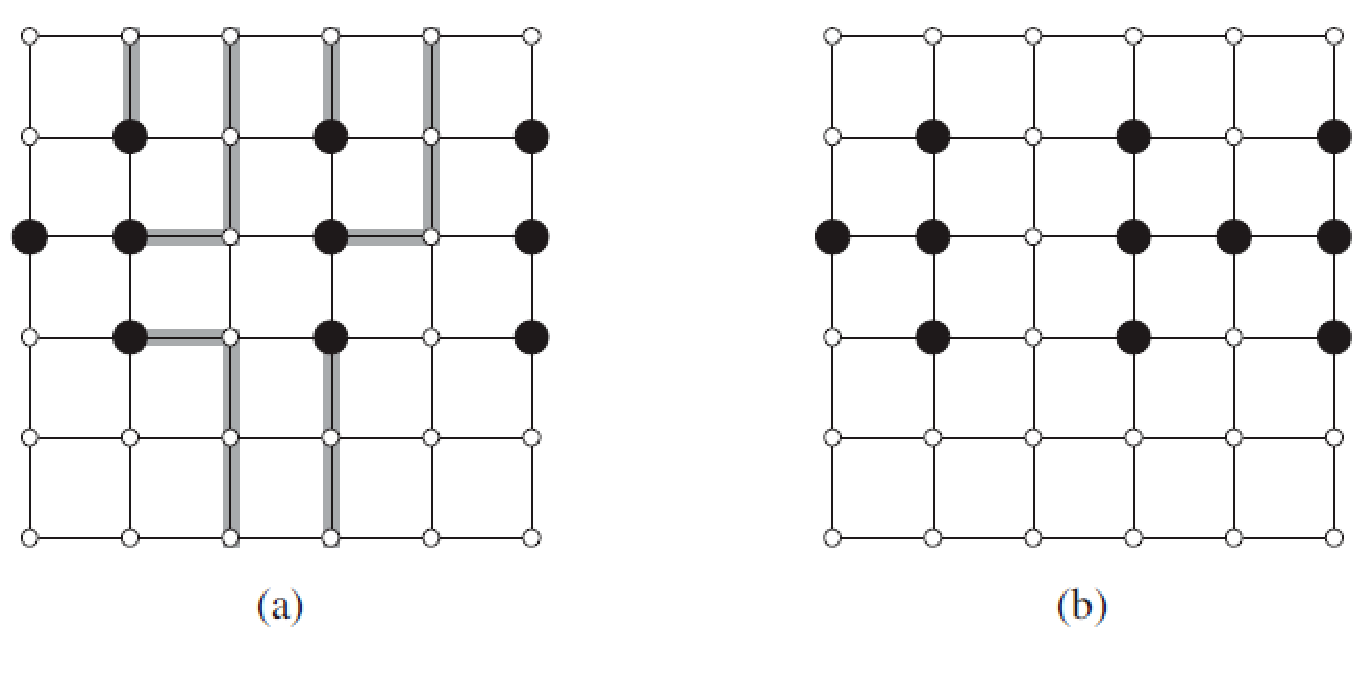
\includegraphics[width=0.5\textwidth]{Fig-EscapeProblem.pdf}
	\caption{Grids for the escape problem. Starting points are black, and other grid vertices are white. (a) A grid with an escape, shown by shaded paths. (b) A grid with no escape.}
	\label{Fig-EscapeProblem}
	\end{figure}
    \begin{enumerate}
        \item Consider a flow network in which vertices, as well as edges, have capacities. That is, the total positive flow entering any given vertex is subject to a capacity constraint. Show that determining the maximum flow in a network with edge and vertex capacities can be reduced to an ordinary maximum-flow problem on a flow network of comparable size. That is, the sizes of the two graph are in the same order of magnitude.
        \item Describe an efficient algorithm to solve the escape problem, and analyze its running time.
    \end{enumerate}

	\begin{solution}
		\begin{enumerate}
			\item We can transfer the maximum flow in a network with edge and vertex capacities to an ordinary maximum-flow problem on a flow network by break up each vertex into two no capacity vertexes. One only receives all the input of the original vertex, the other connects all the output of the original one. And there is a flow from the receiver to the outputer with the capacity the same with the capacity of the original vertex.\\
			After this transition, the number of vertexes doubles, which means the new network is of comparable size of the old one.
			\item The escape problem can be regarded as a flow network with capacible vertexes. Every vertex except the starting points has a capacity of 1. Firstly, all the boundary vertexes can be merged into one vertex without capacity and the connections between boundary vertexes and the other vertexes remain the same with the new vertex. This new vertex is the source vertex of a new and ordinary flow network. Secondly, the remain vertexes except the starting vertexes with capacity of 1 can be transferred into ordinary vertexes with no capacity with the method in problem(a). Thirdly, the starting vertexes can be divided into several parts by neighborhood. Vertexes with the same neighbor starting vertex and the nerghbor itself are a group. Each group is merged into one vertex using the same method of merging bounary vertexes. This new group vertex is a sink with all connections are input. Last, we construct a new vertex connecting all group vertexes, and each connection starts from the group vertex and ends to the new constructed one. each connection has a capacity of the connecting group vertex size. This new constructing vertex is the end vertex of the ordinary flow network. \\
			After this transition, we can solve the escape problem using Ford-Fulkerson Algorithm. And the time complexity is $O((n-1)^2\times n^2)=O(n^4)$.
		\end{enumerate}
	\end{solution}
    
    
\end{enumerate}

\textbf{Remark:} Please include your .pdf, .tex files for uploading with standard file names.
\newpage


%========================================================================
\end{document}